\dummypart{2}{Polynomials}
\myLesson{Polynomial Basics (multiplication)}[2][b]

\begin{myObjectives}
    \myObjective{multiply}{monomials}
\end{myObjectives}
            
\begin{myVocabulary}
    \myDefinition{monomial}{a coefficient times a variable to an \gap{integer} \gap{power}}
    \myDefinition{like terms}{monomials with the variable raised to the \gap{same} \gap{power}}
\end{myVocabulary}

\section{Introduction}

The key to solving absolute value 
\myEmph{equations} was to think about \gap{distance}.

\begin{tcolorbox}[width=4in, center, colback=white,]
    $|x| = 3$
    \tcblower
    \begin{center}
        \begin{tcolorbox}[center,colback=white,boxrule=0.5pt,]
            \small The distance of $x$ from the origin is \myEmph{equal to} $3$.
        \end{tcolorbox}
        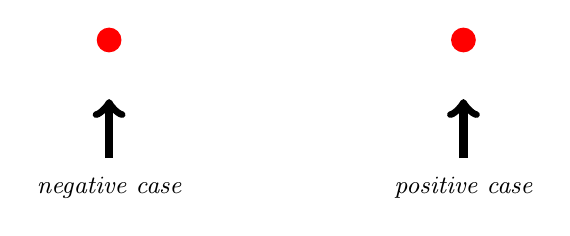
\begin{tikzpicture}[scale=0.75]
            \myDrawNumberlineCircle{0}{white}
            \whenTEACHER{
                % \draw [->,line width=3pt,red] (-3,-2) -- (-3,-1);
                \draw[red,line width=2.5pt,fill=red] (-3,0) circle (0.15 cm);
                %
                % \draw [->,line width=3pt,red] (3,-2) -- (3,-1);
                \draw[red,line width=2.5pt,fill=red] (3,0) circle (0.15 cm);
                }
                \draw[->, black, line width=3pt] (-3,-2) -- (-3,-1);
                \node[] at (-3,-2.5) {\itshape\small negative case};
                \draw[->, black, line width=3pt] (3,-2)  -- (3,-1);
                \node[] at (3,-2.5) {\itshape\small positive case};
                \myDrawNumberline{5}
        \end{tikzpicture}\\
        \whenSTUDENT{\vspace{3\onelineskip}}
        %
        \whenTEACHER{
            {
                $x = -3$
            }
            \hfil
            {
                $x = 3$
            }
        }
    \end{center}
\end{tcolorbox}

Similarly,
the key to solving absolute value
\myEmph{inequalities} is to think about \gap{distance}.


In the last lesson, we added rational expressions. 
We simplified expressions that looked like this.
\[
    \frac
    {(x-2)}
    {(x+3)}
    +
    \frac
    {3x}
    {(x+3)(x+5)}
\]
%
Today we will subtract like this:
\[
    \frac
    {(x-2)}
    {(x+3)}
    \bm{-}
    \frac
    {3x}
    {(x+3)(x+5)}
\]


\begin{tcolorbox}[center,colback=white,width=7in,]
    {\bfseries\itshape Subtraction} 
    is mostly the same as addition.
    The key idea is to combine the fractions 
    over a common \gap{denominator} (LCD).\par
    \vspace{1em}
    But for subtraction, 
    you need to remember to \gap{distribute} the negative.
    This is easy to forget!
\end{tcolorbox}

\begin{myConceptSteps}{To {\bfseries\itshape subtract} two rational expressions\dots}
    \myStep{common denominator}{
        If the fractions have \gap{different} denominators\dots
        \begin{itemize}[nosep]
            \item Factor the denominators.
            \item Find the \gap{LCD} of the two rational expressions.
            \item \gap{Multiply} the numerators and denominators 
            by factors needed to make their denominators equal to the \gap{LCD}.
        \end{itemize}
    }
    \myStep{subtract}{%
        Subtract the \gap{numerators}.
        \begin{itemize}[nosep]
            \item{\bfseries\itshape Do not} subtract the denominators.
            The denominator becomes the \gap{LCD}. 
        \end{itemize}
    }
    \myStep{simplify}{%
        Simplify the expression.
        \begin{itemize}[nosep]
            \item Remember to \gap{distribute} the negative. 
        \end{itemize}
    }
\end{myConceptSteps}


\myWideProblem
    {
        $
        \frac{2x}{x^2+2x-8}
        -
        \frac{1}{2}
        $
    }
    {6.5in}

